% =====================================================================
%  រូបវិទ្យា ថ្នាក់ទី៩ — មេរៀនទី០១ ៖ ការបំបែកកម្លាំង
%  រៀបចំដោយ៖ ពៅ គឹមយ៉ាត — Science Master Academic
%
%  Compile with XeLaTeX (Overleaf: Menu -> Compiler -> XeLaTeX).
%  Requires a Khmer font such as "Noto Serif Khmer" or "Khmer OS Siemreap".
% =====================================================================
\documentclass[12pt,a4paper]{article}

\usepackage{amsmath,amssymb}
\usepackage{fontspec}
\usepackage[a4paper,top=2.6cm,bottom=2.4cm,left=2.3cm,right=2.3cm,headheight=16pt]{geometry}
\usepackage{enumitem}
\usepackage[dvipsnames]{xcolor}
\usepackage{tikz}
\usetikzlibrary{arrows.meta,angles,quotes,calc}
\usepackage[most]{tcolorbox}
\usepackage{titlesec}
\usepackage{fancyhdr}
\usepackage{array,booktabs,colortbl}

% ---- Fonts ----
\setmainfont{Latin Modern Roman}
\newfontfamily\khmerfont[Script=Khmer]{Noto Serif Khmer}
\usepackage[Latin,Khmer]{ucharclasses}
\setTransitionsFor{Khmer}{\khmerfont}{\rmfamily}
\linespread{1.35}

% ---- Colours ----
\definecolor{navy}{HTML}{14325C}
\definecolor{teal}{HTML}{0E7C86}
\definecolor{gold}{HTML}{C9962B}
\definecolor{crimson}{HTML}{B3263A}
\definecolor{forest}{HTML}{2E7D4F}
\definecolor{violet}{HTML}{5B3A8C}
\definecolor{paper}{HTML}{F5F8FC}
\definecolor{softteal}{HTML}{E6F4F5}
\definecolor{softgold}{HTML}{FBF4E4}
\definecolor{softred}{HTML}{FBECEE}
\definecolor{softgreen}{HTML}{E9F5EE}
\definecolor{softviolet}{HTML}{F1ECF8}
\definecolor{inkgray}{HTML}{4A5563}

% ---- Section headings ----
\titleformat{\section}
  {\Large\bfseries\color{navy}}
  {\tikz[baseline=(n.base)]\node[fill=teal,text=white,rounded corners=3pt,
     inner sep=4pt,minimum width=1.6em](n){\thesection};}
  {0.6em}{}[{\color{gold}\titlerule[1.2pt]}]
\titleformat{name=\section,numberless}
  {\Large\bfseries\color{navy}}{}{0pt}{}[{\color{gold}\titlerule[1.2pt]}]
\titlespacing*{\section}{0pt}{1.3em}{0.8em}
\titleformat{\subsection}{\large\bfseries\color{teal}}{\thesubsection}{0.5em}{}
\renewcommand{\thesubsection}{\thesection.\arabic{subsection}}

% ---- Header / footer ----
\pagestyle{fancy}
\fancyhf{}
\fancyhead[L]{\small\color{navy}\textbf{Science Master Academic}}
\fancyhead[R]{\small\color{teal}រូបវិទ្យា ថ្នាក់ទី៩ · មេរៀនទី០១}
\fancyfoot[C]{\tikz\node[fill=navy,text=white,circle,inner sep=2.5pt,
  minimum size=1.5em,font=\small\bfseries]{\thepage};}
\fancyfoot[R]{\scriptsize\color{inkgray}ពៅ គឹមយ៉ាត}
\renewcommand{\headrulewidth}{0.8pt}
\renewcommand{\headrule}{{\color{gold}\hrule height\headrulewidth width\headwidth}}

% ---- Boxes ----
\tcbset{
  base/.style={enhanced,breakable,arc=3pt,boxrule=0pt,left=10pt,right=10pt,
    top=6pt,bottom=6pt,fonttitle=\bfseries,coltitle=white,
    before skip=10pt,after skip=10pt}
}
\newcounter{ex}
\newtcolorbox{objective}{base,colback=softviolet,colframe=violet,
  borderline west={4pt}{0pt}{violet},title={គោលបំណងមេរៀន},
  attach boxed title to top left={xshift=8pt,yshift=-2mm},
  boxed title style={colback=violet,arc=2pt,boxrule=0pt}}
\newtcolorbox{definition}[1][]{base,colback=softteal,colframe=teal,
  borderline west={4pt}{0pt}{teal},
  title={និយមន័យ\ifx\relax#1\relax\else\ ៖ #1\fi},
  attach boxed title to top left={xshift=8pt,yshift=-2mm},
  boxed title style={colback=teal,arc=2pt,boxrule=0pt}}
\newtcolorbox{formula}[1][]{base,colback=softred,colframe=crimson,boxrule=1.2pt,
  title={រូបមន្ត\ifx\relax#1\relax\else\ ៖ #1\fi},
  attach boxed title to top center={yshift=-2mm},
  boxed title style={colback=crimson,arc=2pt,boxrule=0pt}}
\newtcolorbox{note}{base,colback=softgold,colframe=gold,
  borderline west={4pt}{0pt}{gold},title={ចំណាំ},
  attach boxed title to top left={xshift=8pt,yshift=-2mm},
  boxed title style={colback=gold,arc=2pt,boxrule=0pt}}
\newtcolorbox{example}{base,colback=paper,colframe=navy,boxrule=0.8pt,
  title={\stepcounter{ex}ឧទាហរណ៍ទី \theex},
  attach boxed title to top left={xshift=8pt,yshift=-2mm},
  boxed title style={colback=navy,arc=2pt,boxrule=0pt}}
\newtcolorbox{solution}{enhanced,breakable,arc=0pt,boxrule=0pt,
  colback=white,colframe=white,left=12pt,right=8pt,top=2pt,bottom=2pt,
  borderline west={2pt}{0pt}{teal!70},before skip=4pt,after skip=12pt,
  before upper={{\color{teal}\bfseries ដំណោះស្រាយ ៖}\par}}
\newtcolorbox{summary}{base,colback=softgreen,colframe=forest,boxrule=1.2pt,
  title={សេចក្តីសង្ខេប},attach boxed title to top center={yshift=-2mm},
  boxed title style={colback=forest,arc=2pt,boxrule=0pt}}

\newcommand{\keyformula}[1]{%
  \begin{center}\tcbox[enhanced,colback=white,colframe=crimson,boxrule=1.2pt,
    arc=4pt,left=10pt,right=10pt,top=4pt,bottom=4pt]{$\displaystyle #1$}\end{center}}
\newcommand{\ans}[1]{{\color{crimson}\boxed{#1}}}
\newcommand{\vF}{\vec{F}}
\newcommand{\unit}[1]{\,\mathrm{#1}}

\begin{document}

% =====================================================================
%  TITLE BANNER
% =====================================================================
\thispagestyle{empty}
\begin{tikzpicture}[remember picture,overlay]
  \fill[navy] (current page.north west) rectangle ([yshift=-7.2cm]current page.north east);
  \fill[teal] ([yshift=-7.2cm]current page.north west) rectangle ([yshift=-7.6cm]current page.north east);
  \fill[gold] ([yshift=-7.6cm]current page.north west) rectangle ([yshift=-7.75cm]current page.north east);
  \node[text=gold,font=\small\bfseries,anchor=north]
     at ([yshift=-1.3cm]current page.north) {SCIENCE MASTER ACADEMIC};
  \node[text=white!85!teal,font=\large,anchor=north]
     at ([yshift=-2.0cm]current page.north) {រូបវិទ្យា ថ្នាក់ទី៩ · មេរៀនទី០១};
  \node[text=white,font=\Huge\bfseries,anchor=north]
     at ([yshift=-3.0cm]current page.north) {ការបំបែកកម្លាំង};
  \node[text=white,font=\Large,anchor=north]
     at ([yshift=-4.9cm]current page.north)
     {$F_x = F\cos\alpha \qquad F_y = F\sin\alpha$};
\end{tikzpicture}
\vspace*{5.4cm}

\begin{center}
\begin{tcolorbox}[enhanced,width=0.62\linewidth,colback=paper,colframe=navy,
  boxrule=0.8pt,arc=4pt,halign=center]
  {\color{inkgray}រៀបចំដោយ}\\[2pt]
  {\Large\bfseries\color{navy}ពៅ គឹមយ៉ាត}\\[2pt]
  {\small\color{teal}Science Master Academic}
\end{tcolorbox}
\end{center}

\begin{objective}
បន្ទាប់ពីរៀនមេរៀននេះចប់ សិស្សអាច៖
\begin{itemize}[leftmargin=1.4em,itemsep=0pt]
  \item ពន្យល់បានថា \textbf{ការបំបែកកម្លាំង} ជាអ្វី ។
  \item បំបែកកម្លាំងមួយជាកម្លាំងពីរកែងគ្នា ដោយ\textbf{គំនូស} និងដោយ\textbf{ការគណនា} ។
  \item ប្រើរូបមន្ត $F_x=F\cos\alpha$ , $F_y=F\sin\alpha$ និង $F=\sqrt{F_x^2+F_y^2}$ ។
  \item បំបែក\textbf{ទម្ងន់}របស់វត្ថុលើ\textbf{ប្លង់ទេរ} ។
\end{itemize}
\end{objective}

% =====================================================================
\section{រំលឹកមេរៀន ៖ កម្លាំង}

កម្លាំង $\vF$ គឺជា\textbf{មហិមាវ៉ិចទ័រ} ដែលមានធាតុ ៤ ៖
\begin{center}
\renewcommand{\arraystretch}{1.3}
\begin{tabular}{>{\columncolor{softteal}\bfseries}l l}
\toprule
\rowcolor{teal}\color{white}ធាតុ & \color{white}\textbf{អត្ថន័យ}\\
\midrule
ចំណុចអនុវត្ត & ចំណុចដែលកម្លាំងមានអំពើលើវត្ថុ\\
ទិស & បន្ទាត់ដែលកម្លាំងមានអំពើតាម (ផ្ដេក បញ្ឈរ ទេរ...)\\
ទិសដៅ & ទៅឆ្វេង/ស្តាំ ឡើងលើ/ចុះក្រោម ...\\
អាំងតង់ស៊ីតេ & តម្លៃនៃកម្លាំង គិតជា \textbf{ញូតុន} ($\mathrm{N}$)\\
\bottomrule
\end{tabular}
\end{center}

% =====================================================================
\section{និយមន័យនៃការបំបែកកម្លាំង}

\begin{definition}[ការបំបែកកម្លាំង]
\textbf{ការបំបែកកម្លាំង} គឺជាការជំនួសកម្លាំងមួយ $\vF$ ដោយកម្លាំងពីរ
$\vF_x$ និង $\vF_y$ ដែលមាន\textbf{អំពើដូចគ្នា}នឹងកម្លាំង $\vF$ ។
\[
  \vF = \vF_x + \vF_y
\]
កម្លាំង $\vF_x$ និង $\vF_y$ ហៅថា \textbf{កម្លាំងបំបែក} (components)
ហើយ $\vF$ ជា\textbf{កម្លាំងផ្គុំ} ។
\end{definition}

\begin{note}
ការបំបែកកម្លាំង គឺជាប្រមាណវិធី\textbf{ច្រាស}នៃការផ្គុំកម្លាំង ។
គេប្រើ\textbf{វិធានប្រលេឡូក្រាម} ៖ $\vF$ ជាអង្កត់ទ្រូងនៃប្រលេឡូក្រាម
ដែលមានជ្រុងជាប់គ្នាជា $\vF_x$ និង $\vF_y$ ។
\end{note}

% =====================================================================
\section{វិធីបំបែកកម្លាំងជាពីរកែងគ្នា}

\subsection{វិធីគំនូស}
\begin{enumerate}[leftmargin=1.6em,itemsep=2pt]
  \item គូសអ័ក្ស $Ox$ (ផ្ដេក) និង $Oy$ (បញ្ឈរ) កាត់តាមចំណុចអនុវត្ត $O$ ។
  \item ពីចុងវ៉ិចទ័រ $\vF$ គូសបន្ទាត់\textbf{កែង}ទៅលើអ័ក្សនីមួយៗ ។
  \item ចំណោលលើ $Ox$ គឺ $\vF_x$ ហើយចំណោលលើ $Oy$ គឺ $\vF_y$ ។
\end{enumerate}

\begin{center}
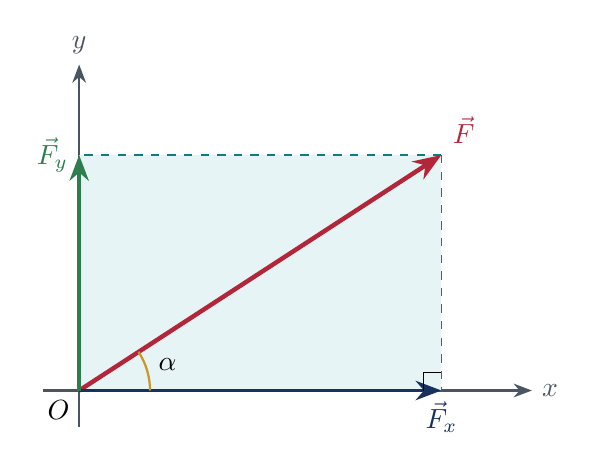
\begin{tikzpicture}[scale=1.15,>=Stealth]
  \draw[->,thick,inkgray] (-0.4,0) -- (5,0) node[right]{$x$};
  \draw[->,thick,inkgray] (0,-0.4) -- (0,3.6) node[above]{$y$};
  \coordinate (O) at (0,0);
  \coordinate (F) at (4,2.6);
  \coordinate (Fx) at (4,0);
  \coordinate (Fy) at (0,2.6);
  \fill[softteal] (O) -- (Fx) -- (F) -- (Fy) -- cycle;
  \draw[dashed,teal] (F) -- (Fx);
  \draw[dashed,teal] (F) -- (Fy);
  \draw[->,line width=1.6pt,crimson] (O) -- (F) node[above right]{$\vF$};
  \draw[->,line width=1.4pt,navy] (O) -- (Fx) node[below]{$\vF_x$};
  \draw[->,line width=1.4pt,forest] (O) -- (Fy) node[left]{$\vF_y$};
  \pic[draw=gold,thick,"$\alpha$",angle radius=0.9cm,angle eccentricity=1.3] {angle=Fx--O--F};
  \draw (3.8,0) -- (3.8,0.2) -- (4,0.2);
  \node[below left] at (O){$O$};
\end{tikzpicture}
\end{center}

\subsection{វិធីគណនា}
ក្នុងត្រីកោណកែង ដែលមានអ៊ីប៉ូតេនុស $F$ និងមុំ $\alpha$ រវាង $\vF$ និងអ័ក្ស $Ox$ ៖

\begin{formula}[ការបំបែកកម្លាំង]
\[
  \boxed{F_x = F\cos\alpha}\qquad\qquad \boxed{F_y = F\sin\alpha}
\]
\end{formula}

\begin{formula}[រកកម្លាំងផ្គុំពីកម្លាំងបំបែក]
\[
  \boxed{F=\sqrt{F_x^{2}+F_y^{2}}}\qquad\qquad
  \boxed{\tan\alpha=\dfrac{F_y}{F_x}}
\]
\end{formula}

\begin{center}
\renewcommand{\arraystretch}{1.35}
\begin{tabular}{>{\columncolor{softgold}\bfseries}c c c c c c}
\toprule
\rowcolor{gold}\color{white}$\alpha$ & \color{white}$0^\circ$ & \color{white}$30^\circ$
 & \color{white}$45^\circ$ & \color{white}$60^\circ$ & \color{white}$90^\circ$\\
\midrule
$\sin\alpha$ & $0$ & $\tfrac12=0.5$ & $\tfrac{\sqrt2}{2}\approx0.71$ & $\tfrac{\sqrt3}{2}\approx0.87$ & $1$\\
$\cos\alpha$ & $1$ & $\tfrac{\sqrt3}{2}\approx0.87$ & $\tfrac{\sqrt2}{2}\approx0.71$ & $\tfrac12=0.5$ & $0$\\
\bottomrule
\end{tabular}

{\small\color{inkgray}(គេអាចប្រើ $\sin37^\circ\approx0.6$ និង $\cos37^\circ\approx0.8$)}
\end{center}

% =====================================================================
\section{ការបំបែកទម្ងន់លើប្លង់ទេរ}

វត្ថុមួយដែលមានម៉ាស $m$ ដាក់លើប្លង់ទេរ ដែលមានមុំទេរ $\alpha$ ។
ទម្ងន់ $\vec P$ ($P=mg$) ត្រូវបានបំបែកជាពីរ ៖
\begin{itemize}[leftmargin=1.4em,itemsep=0pt]
  \item $\vec P_{\parallel}$ ៖ ស្របនឹងប្លង់ទេរ (ធ្វើឲ្យវត្ថុរអិលចុះ)
  \item $\vec P_{\perp}$ ៖ កែងនឹងប្លង់ទេរ (សង្កត់លើប្លង់)
\end{itemize}

\begin{center}
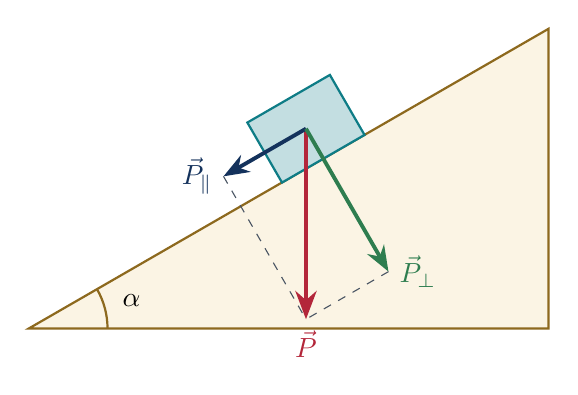
\begin{tikzpicture}[scale=1.1,>=Stealth]
  \coordinate (A) at (0,0);
  \coordinate (B) at (6,0);
  \coordinate (C) at (6,3.46);
  \fill[softgold] (A) -- (B) -- (C) -- cycle;
  \draw[thick,gold!70!black] (A) -- (B) -- (C) -- cycle;
  \pic[draw=gold!70!black,thick,"$\alpha$",angle radius=1cm,angle eccentricity=1.35] {angle=B--A--C};
  % block on incline
  \begin{scope}[shift={(3.4,1.96)},rotate=30]
    \fill[teal!25] (-0.55,0) rectangle (0.55,0.8);
    \draw[thick,teal] (-0.55,0) rectangle (0.55,0.8);
    \coordinate (G) at (0,0.4);
  \end{scope}
  \draw[->,line width=1.6pt,crimson] (G) -- ++(0,-2.2) node[below]{$\vec P$};
  \draw[->,line width=1.4pt,navy] (G) -- ++(210:1.1) node[left]{$\vec P_{\parallel}$};
  \draw[->,line width=1.4pt,forest] (G) -- ++(-60:1.905) node[right]{$\vec P_{\perp}$};
  \draw[dashed,inkgray] ($(G)+(210:1.1)$) -- ($(G)+(0,-2.2)$);
  \draw[dashed,inkgray] ($(G)+(-60:1.905)$) -- ($(G)+(0,-2.2)$);
\end{tikzpicture}
\end{center}

\begin{formula}[ទម្ងន់លើប្លង់ទេរ]
\[
  P = mg \qquad\quad
  \boxed{P_{\parallel}=P\sin\alpha} \qquad\quad
  \boxed{P_{\perp}=P\cos\alpha}
\]
\end{formula}

\begin{note}
មុំរវាង $\vec P$ និង $\vec P_{\perp}$ ស្មើនឹងមុំទេរ $\alpha$ ។
ដូច្នេះ $P_{\parallel}$ ប្រើ $\sin$ ហើយ $P_{\perp}$ ប្រើ $\cos$ ។
យក $g=10\unit{N/kg}$ ។
\end{note}

% =====================================================================
\section{ឧទាហរណ៍គំរូ}

\begin{example}
កម្លាំង $F=10\unit N$ ធ្វើមុំ $\alpha=30^\circ$ ជាមួយអ័ក្សផ្ដេក ។
គណនាកម្លាំងបំបែក $F_x$ និង $F_y$ ។
\end{example}
\begin{solution}
\[
  F_x = F\cos30^\circ = 10\times\frac{\sqrt3}{2}\approx \ans{8.66\unit N},
  \qquad
  F_y = F\sin30^\circ = 10\times\frac12 = \ans{5\unit N}.
\]
\end{solution}

\begin{example}
កម្លាំងបំបែកពីរកែងគ្នា $F_x=6\unit N$ និង $F_y=8\unit N$ ។
រកអាំងតង់ស៊ីតេនៃកម្លាំងផ្គុំ $F$ និងមុំ $\alpha$ ដែល $\vF$ ធ្វើជាមួយអ័ក្ស $Ox$ ។
\end{example}
\begin{solution}
\[
  F=\sqrt{6^2+8^2}=\sqrt{100}=\ans{10\unit N},
  \qquad
  \tan\alpha=\frac{8}{6}=\frac43 \;\Rightarrow\; \alpha\approx\ans{53^\circ}.
\]
\end{solution}

\begin{example}
សិស្សម្នាក់ទាញរទេះដោយខ្សែ ដែលធ្វើមុំ $60^\circ$ ជាមួយផ្ទៃដី ដោយកម្លាំង
$F=40\unit N$ ។ រកកម្លាំងដែលទាញរទេះទៅមុខ និងកម្លាំងដែលលើករទេះឡើងលើ ។
\end{example}
\begin{solution}
\begin{itemize}[leftmargin=1.4em,itemsep=0pt]
  \item កម្លាំងទាញទៅមុខ (ផ្ដេក)៖ $F_x=40\cos60^\circ=40\times0.5=\ans{20\unit N}$
  \item កម្លាំងលើកឡើងលើ (បញ្ឈរ)៖ $F_y=40\sin60^\circ=40\times\dfrac{\sqrt3}{2}\approx\ans{34.6\unit N}$
\end{itemize}
\end{solution}

\begin{example}
ប្រអប់មួយម៉ាស $m=5\unit{kg}$ ស្ថិតលើប្លង់ទេរ ដែលមានមុំទេរ $\alpha=30^\circ$ ។
($g=10\unit{N/kg}$) គណនា $P$ , $P_{\parallel}$ និង $P_{\perp}$ ។
\end{example}
\begin{solution}
\[
  P = mg = 5\times10 = \ans{50\unit N}
\]
\[
  P_{\parallel}=P\sin30^\circ=50\times0.5=\ans{25\unit N},
  \qquad
  P_{\perp}=P\cos30^\circ=50\times\frac{\sqrt3}{2}\approx\ans{43.3\unit N}.
\]
\end{solution}

% =====================================================================
\section{លំហាត់អនុវត្ត}

\newcommand{\qnum}[1]{\tikz[baseline=(c.base)]\node[fill=teal,text=white,
  circle,inner sep=1.5pt,minimum size=1.3em,font=\small\bfseries](c){#1};}
\begin{enumerate}[label=\protect\qnum{\arabic*},leftmargin=2.4em,itemsep=8pt]
  \item កម្លាំង $F=20\unit N$ ធ្វើមុំ $45^\circ$ ជាមួយអ័ក្សផ្ដេក ។
        គណនា $F_x$ និង $F_y$ ។
  \item កម្លាំង $F=50\unit N$ ធ្វើមុំ $37^\circ$ ជាមួយអ័ក្សផ្ដេក ។
        គណនា $F_x$ និង $F_y$ ។ (យក $\sin37^\circ=0.6$ , $\cos37^\circ=0.8$)
  \item កម្លាំងបំបែក $F_x=12\unit N$ និង $F_y=5\unit N$ ។
        រកកម្លាំងផ្គុំ $F$ ។
  \item កម្លាំង $F=30\unit N$ ធ្វើមុំ $60^\circ$ ជាមួយអ័ក្សបញ្ឈរ ។
        គណនាកម្លាំងបំបែកផ្ដេក និងបញ្ឈរ ។
  \item ប្រអប់ម៉ាស $m=2\unit{kg}$ ដាក់លើប្លង់ទេរ $\alpha=37^\circ$ ។
        ($g=10\unit{N/kg}$) គណនា $P$ , $P_{\parallel}$ និង $P_{\perp}$ ។
  \item កម្លាំង $F$ មួយមានកម្លាំងបំបែកផ្ដេក $F_x=15\unit N$ និងធ្វើមុំ
        $60^\circ$ ជាមួយអ័ក្សផ្ដេក ។ រក $F$ និង $F_y$ ។
\end{enumerate}

% =====================================================================
\section*{ចម្លើយលំហាត់}
\begin{tcolorbox}[base,colback=paper,colframe=inkgray!40,boxrule=0.6pt]
\renewcommand{\arraystretch}{1.5}
\begin{tabular}{@{}r@{\quad}l@{}}
\qnum{1} & $F_x=F_y=20\times0.71\approx14.1\unit N$\\
\qnum{2} & $F_x=50\times0.8=40\unit N$ , \ $F_y=50\times0.6=30\unit N$\\
\qnum{3} & $F=\sqrt{12^2+5^2}=\sqrt{169}=13\unit N$\\
\qnum{4} & មុំជាមួយផ្ដេក $=90^\circ-60^\circ=30^\circ$ ៖
           $F_x=30\cos30^\circ\approx26\unit N$ , \ $F_y=30\sin30^\circ=15\unit N$\\
\qnum{5} & $P=20\unit N$ , \ $P_{\parallel}=20\times0.6=12\unit N$ , \
           $P_{\perp}=20\times0.8=16\unit N$\\
\qnum{6} & $F=\dfrac{F_x}{\cos60^\circ}=\dfrac{15}{0.5}=30\unit N$ , \
           $F_y=30\sin60^\circ\approx26\unit N$\\
\end{tabular}
\end{tcolorbox}

% =====================================================================
\begin{summary}
\begin{itemize}[leftmargin=1.4em,itemsep=2pt]
  \item ការបំបែកកម្លាំង ៖ ជំនួស $\vF$ ដោយកម្លាំងពីរ ដែល $\vF=\vF_x+\vF_y$ ។
  \item កម្លាំងបំបែកកែងគ្នា ៖ $F_x=F\cos\alpha$ , \ $F_y=F\sin\alpha$
        ($\alpha$ ជាមុំជាមួយអ័ក្ស $Ox$) ។
  \item ពីកម្លាំងបំបែក ៖ $F=\sqrt{F_x^2+F_y^2}$ , \ $\tan\alpha=\dfrac{F_y}{F_x}$ ។
  \item លើប្លង់ទេរ ៖ $P_{\parallel}=mg\sin\alpha$ , \ $P_{\perp}=mg\cos\alpha$ ។
\end{itemize}
\end{summary}

\vspace{0.8cm}
\begin{flushright}
\begin{tabular}{r}
{\color{inkgray}រៀបចំដោយ}\\
{\large\bfseries\color{navy}ពៅ គឹមយ៉ាត}\\
{\color{gold}\rule{4.5cm}{1pt}}\\
{\small\color{teal}Science Master Academic}
\end{tabular}
\end{flushright}

\end{document}
